\chapter{Hash Functions}

\section{Introduction}

A hash function takes a variable sized input message and produces a fixed-sized output. Every cryptographic hash function is a hash function. Not every hash function is a cryptographic hash function. Non-cryptographic hash functions try to avoid collisions for (non-malicious) input. Cryptographic hash function need to be very fast to compute, have a very low probability of collisions and it has to be computationally infeasible to invert (e.g. given an hash say what was the value that generated that hash).

The digest can be seen as a fixed-sized fingerprint of a variable-sized message. Since a message digest depends on all the bits in the input message, any alteration of the input message during transmission would cause its message digest to not match with its original message digest.

\section{Characterizing cryptographic hash functions}

A hash function is called cryptographically secure if it is computationally infeasible to find:
\begin{itemize}
	\item a message that corresponds to a given digest, this is called the one-way property of a hash function. Remark: a hash function must possess this property regardless of the length of the messages. It should be just as difficult to recover from its digest a message that is as short as, a single byte as a message that consists of millions of bytes.
	\item two different messages that hash to the same digest, this is called the strong collision resistance property of a hash function.
\end{itemize}

Both of these conditions need to be true. A weaker form of the strong collision resistance property is that for a given message, there should not correspond another message with the same digest. This is called the weak collision resistance property of a hash function. Collision resistance refers to the likelihood that two different messages will result in the same digest. If the digest produced by a hash function consists of $n$ bits, then there are only $2^n$ distinct digests. If we place no constraints on the messages and if there can be an arbitrary number of different possible messages, then obviously there will exist multiple messages giving rise to the same diges. An example cryptographic hash function is SHA-512.

\section{Applications of Hash functions}

The main applications are authenticity \ref{fig:hashauthentication} and integrity.

\begin{figure}
	\centering
	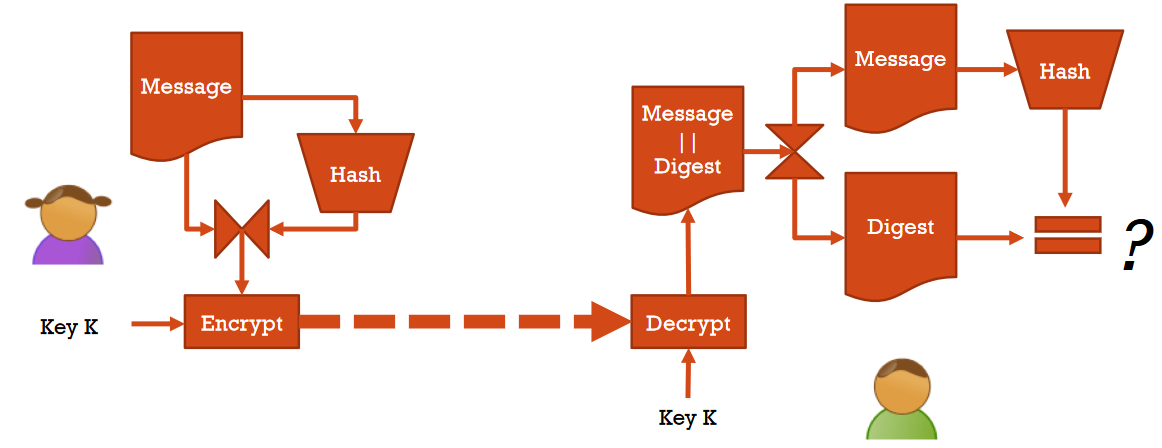
\includegraphics[width=0.7\linewidth]{Images/Chapter6/hash_authentication}
	\caption{Hash functions for message authentication}
	\label{fig:hashauthentication}
\end{figure}

We assume that symmetric key cryptography is used.
\begin{itemize}
	\item Both Alice and Bob use the same shared key $\mathcal{K}$
	\item Alice concatenates the message and its digest to form a composite message that is then encrypted and sent over the network
	\item Bob decrypts the message and separates out its digest, which is then compared with the digest calculated from the received message
	\item The digest provides authentication and the encryption provides confidentiality
\end{itemize}

\begin{figure}
	\centering
	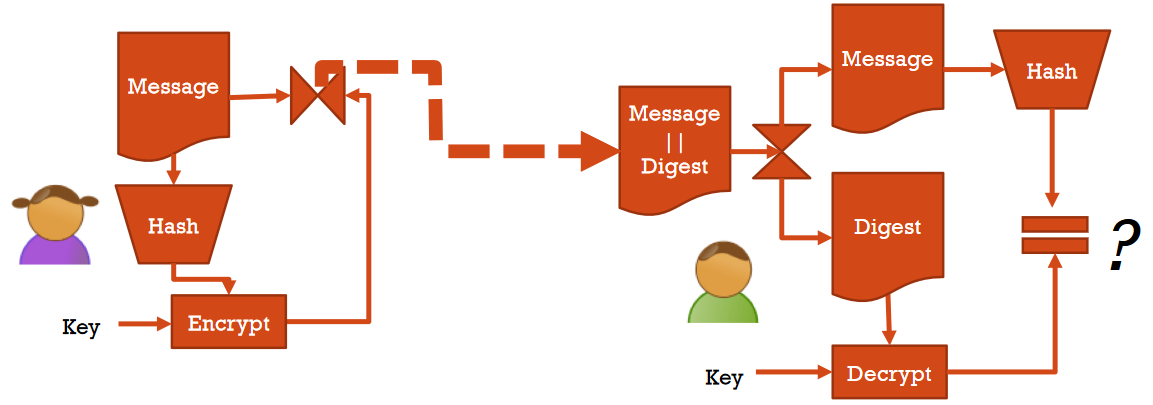
\includegraphics[width=0.7\linewidth]{Images/Chapter6/hash_authentication2}
	\caption{Hash functions for message authentication (2)}
	\label{fig:hashauthentication2}
\end{figure}


Interpretation 1: symmetric key cryptography is used  \ref{fig:hashauthentication2}
\begin{itemize}
	\item Variant of previous schema where only the digest is encrypted
	\item This scheme is efficient to use when confidentiality is not an issue but message authentication is critical
	\item Only the receiver with access to the secret key knows the real digest for the message and can verify whether or not the message is authentic
	\item A digest produced in this way is known as the Message Authentication Code (MAC) and the hash function producing it as a keyed hash function (more on this below)
\end{itemize}

Interpretation 2: public key cryptography is used \ref{fig:hashauthentication2}
\begin{itemize}
	\item Alice uses its private key while Bob uses Alice public key
	\item Confidentiality is not considered
	\item The sender encrypting with its private key the digest of the message constitutes the basic idea of digital signatures, as explained in previous lectures
\end{itemize}


\begin{figure}
	\centering
	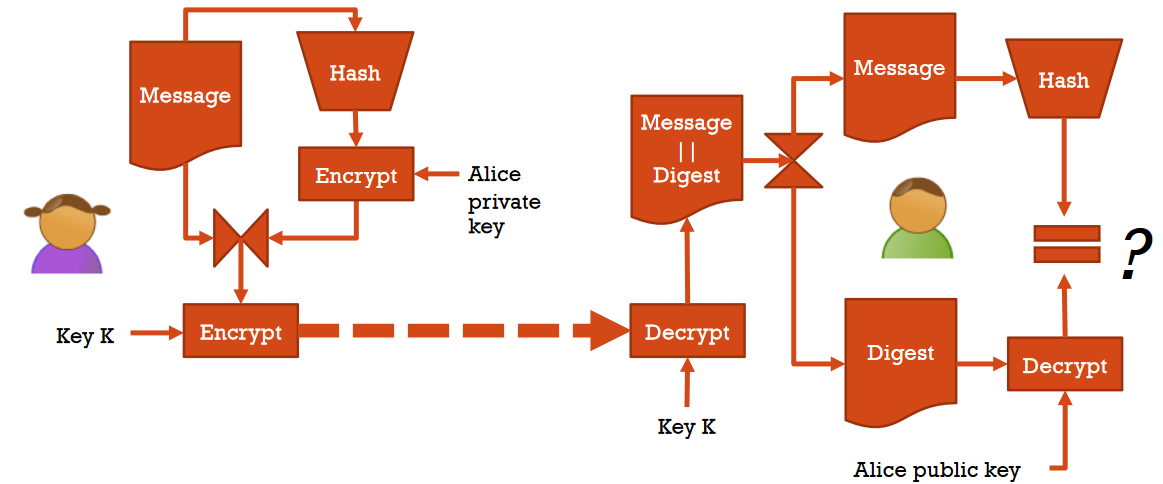
\includegraphics[width=0.7\linewidth]{Images/Chapter6/hash_authentication3}
	\caption{Hash functions for message authentication (3)}
	\label{fig:hashauthentication3}
\end{figure}

We assume the availability of both public and symmetric key cryptography \ref{fig:hashauthentication3}.
\begin{itemize}
	\item Commonly used approach when both confidentiality and authentication are important
	\item Alice encrypts the digest of the message with its private key, concatenates it with the message and then encrypts the result with the shared key
	\item  Bob decrypts the received message with the shared key, calculates the digest from the extracted message and compares it with the decrypted digest by using Alice public key
\end{itemize}


\begin{figure}
	\centering
	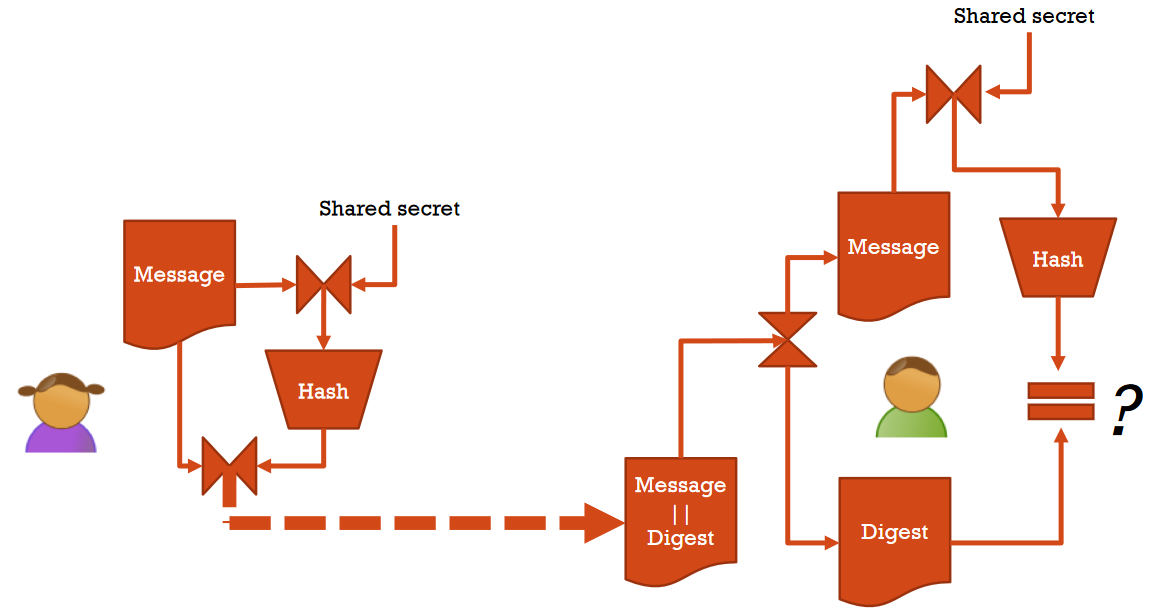
\includegraphics[width=0.7\linewidth]{Images/Chapter6/hash_authentication4}
	\caption{Hash functions for message authentication (4)}
	\label{fig:hashauthentication4}
\end{figure}

We do not need to assume the availability of neither public nor symmetric key cryptography \ref{fig:hashauthentication4}.
\begin{itemize}
	\item In this scheme, no message is encrypted
	\item Alice appends a shared secret string known also to Bob, to the message before computing its digest
	\item Before checking the digest of the received message for its authentication, Bob appends the same shared secret string to the message
	\item It would not be possible for anyone to alter such a message, even when they have access to both the original message and the overall digest
	\item Notice that in this case, confidentiality is not considered
\end{itemize}

\begin{figure}
	\centering
	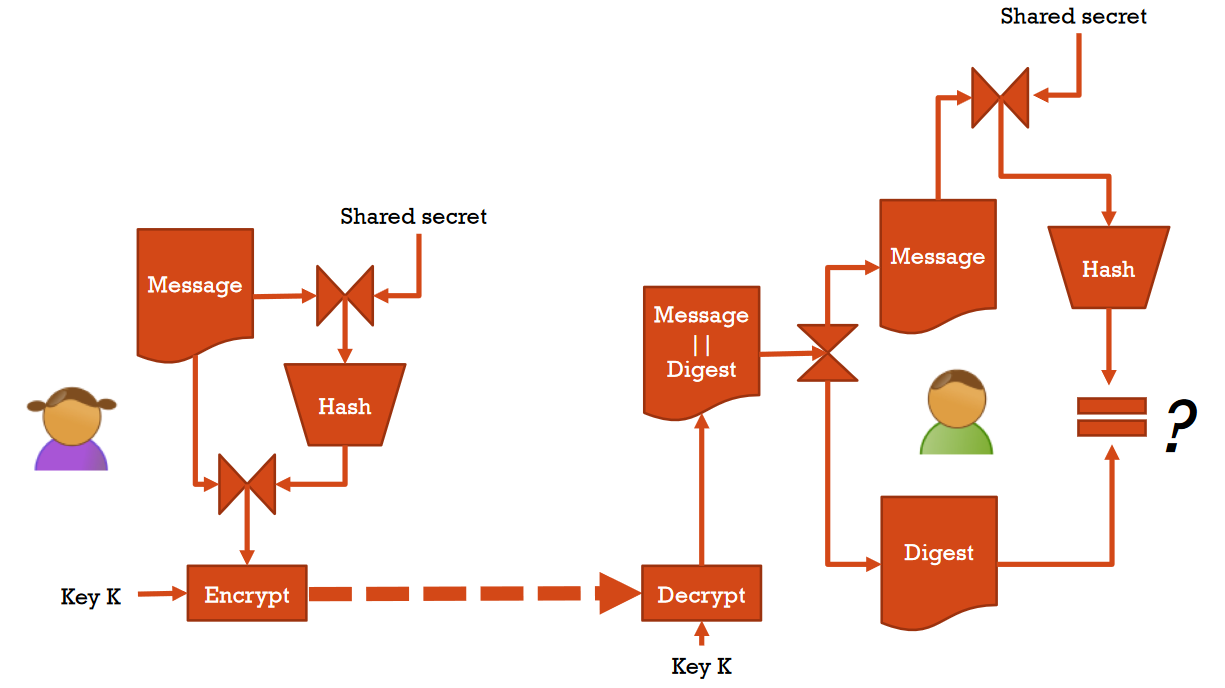
\includegraphics[width=0.7\linewidth]{Images/Chapter6/hash_authentication5}
	\caption{Hash functions for message authentication (5)}
	\label{fig:hashauthentication5}
\end{figure}

We assume the availability of symmetric key cryptography \ref{fig:hashauthentication5}.
\begin{itemize}
	\item This scheme is similar to the previous one with the addition of symmetric key cryptography for confidentiality
	\item Alice appends a shared secret string known also to Bob, to the message before computing its digest
	\item Before checking the digest of the received message for its authentication, Bob appends the same shared secret string to the message
	\item It would not be possible for anyone to alter such a message, even when they have access to both the original message and the overall digest
\end{itemize}


\section{Authenticated encryption with additional data (AEAD)}

When using symmetric ciphers, it is crucial to avoid replay attacks. For example assume Alice sends a message to Bob containing "You can take holidays tomorrow" encrypted with key $K$. An Bob takes holidays as expected. The next day the attacker replays the message and Bob takes another day of vacation, and Alice is left wondering why Bob is not at work.

To avoid the replay attack, what is needed is to bind the cipher to a network connection or a session, in order that Eve cannot recreate the same scenario. With enhanced encryption methods, known as Authenticated Encryption with Associated Data (AEAD), it is possible to both authenticate the cipher and prove its integrity. For this we provide additional data to authenticate the encryption process, and where we can identify where the ciphertext has been modified, and for it not to be decrypted. With most conventional AEAD methods we create a nonce value and add additional data (AD) that is authenticated but not encrypted. Additional data can include addresses, ports, sequence numbers, protocol version.
Additional Data allows for binding network packets to the encrypted data, and provide integrity, so that an intruder cannot copy and paste valid ciphertext from other transmissions. If we bind to a packet sequence number and the port, the authentication would fail for another sequence number or another port.  Indeed, the wider the range of additional data, the more difficult it will be for an attacker to replicate it.  Examples of AEAD are AES-GCM and ChaCha20/Poly1305.

Encryption takes as input the plaintext, key, and optionally a header in plaintext that will no be encrypted, but will be covered by authenticity protection. Its output is the ciphertext and authentication tag (Message Authentication or MAC).
Decryption takes as input the ciphertext, key, authentication tag, and optionally a header (if used during the encryption). Its output is the plaintext, or an error if the authentication tag does not match the supplied ciphertext or header.
The header part is intended to provide authenticity and integrity protection for networking or storage metadata for which confidentiality is unnecessary, but authenticity is desired.

The need for authenticated encryption emerged from the observation that securely combining separate confidentiality and authentication block cipher operation modes could be error prone and difficult.
This was confirmed by a number of practical attacks introduced into production protocols and applications by incorrect implementation, or lack of authentication (including SSL/TLS).

\section{Structure of hash functions}

All algorithms for computing the digest of a message view it as a sequence of $n$-bit blocks. The message is processed one block at a time in an iterative fashion in order to generate its digest. The simplest hash function consists of starting with the first $n$-bit block, perform the bitwise xor with the second $n$-bit block perform the bitwise xor with the next $n$-bit block and so on... This procedure is known as the xor algorithm or the longitudinal parity check as every bit of the digest represents the parity at that bit position if we look across all of the $n$-bit blocks.
The digest generated by the xor algorithm can be useful as a data integrity check in the presence of completely random transmission errors. In the presence of an adversary trying to deliberately tamper with the message content, the xor algorithm is useless for message authentication. An adversary can modify the main message and add a suitable bit block before the digest so that the final digest remains unchanged.

When hashing regular text and the character encoding is based on ASCII, the
collision resistance property of the xor algorithm suffers even more because the highest bit in every byte will be zero. Ideally, one would hope that, with an $n$-bit digest, any particular message would result in a given digest value with a probability of $2^{-n}$. When the highest bit in each byte for each character is always 0, some of the n bits in the digest will predictably be 0 with the xor algorithm. This reduces the number of unique digests available and thus increases the probability of collisions.
An attempt to avoid this problem is a variation on the basic xor algorithm that consists of performing a one-bit circular shift of the partial digest obtained after each $n$-bit block of the message is processed, this algorithm is known as the rotated XOR, but it suffers to a similar problem. XOR should be avoided as the right way out is to include the length of the message in the digest.

\section{Birthday attack}
We are interested in computing the probability that any of the messages is going to have its digest equal to a particular value $h$. More formally: given a pool of $k$ messages produced randomly by the message generator, what is the value of $k$ so that the pool contains at least one message whose digest is equal to $h$ with probability $1/2$?

To establish $k$ consider that the digest can take on $N$ different but equiprobable values, and pick a message $x$ at random from the pool of messages. Since all $N$ digests are equiprobable, the probability of a message $x$ having its digest equal to $h$ is $\frac{1}{N}$. Since the digest of message $x$ is either equal to $h$ or not, the probability of the latter is $1 - (\frac{1}{N})$.  If we pick, say, two messages $x$ and $y$ randomly from the pool, the events that the digest of neither is equal to $h$ are probabilistically independent. This implies that the probability that none of two messages has its digest equal to $h$ is $(1 - (\frac{1}{N}))^2$. More generally, in a pool of $k$ messages, the probability that none of the messages in a pool of $k$ messages has its digest equal to $h$ is  $(1 - (\frac{1}{N}))^k$. Thus the probability that at least one of the $k$ messages has its digest equal to $h$ is $1 - (1 - \frac{1}{N})^k$. This can be simplified to $\frac{k}{N}$ by observing that $(1 + a)^n \approx 1 + a * n$ as $n$ gets close to $0$. So, given a pool of $k$ randomly produced messages, the probability there will exist at least one message in this pool whose digest is equal to a given value $h$ is $\frac{k}{N}$. To answer the original question it is sufficient to solve the equation $\frac{k}{N} = 1/2$ i.e. $k = \frac{N}{2}$.

Consider a digest of 64 bits, then $N = 2^{64}$ and $k = N / 2 = 2^{63}$, so we must construct a pool of $2^{63}$ messages so to be able to find in it a digest equal to $h$ with probability of $50\%$.

In a more friendlier way, what is the probability that, in a class of 20 students, someone else has the same birthday as yours? The answer is $19/365 = 5.2\%$..

Next, we are interested in computing, given a pool of randomly selected messages, the probability that at least two messages in the pool have the same digest. More precisely: given a pool of $k$ messages produced randomly by the message generator, what is the probability that there exist at least two messages in the pool with the same digest?

Let $M_1$ be be the total number of ways in which we can construct a pool of k message with no duplicate digests. Let $M_2$ be the total number of ways in which we can construct a pool of k messages allowing for duplicates. Then $\frac{M_1}{M_2}$ is the the probability of constructing a pool of $k$ messages with no duplicates. Subtracting this from $1$ yields the probability that the pool of $k$ messages will have at least one duplicate digest.
For $M_1$ we need to find out in how many different ways we can construct a pool of $k$ messages so that we are guaranteed to have no duplicate digests in the pool. For the first message there are $N$ different candidates, for the second $N-1$ and so on, so in total $N * (N-1) * \ldots * (N-k+1)$ that is equivalent to \[\binom{N}{k} = \frac{N!}{(N-k)!}\]

For $M_2$ we need to figure out he total number of ways in which we can construct a pool of $k$ messages without worrying at all about duplicate digests. There are $N$ ways to choose the first message to insert in the pool, for the second message there are still $N$ ways, so in total $N^k$.

Thus we have: \[\frac{M_1}{M_2} = \frac{N!}{(N-k)! * N^k} \].
To answer our question of the probability that the pool of k elements has at least one duplication in the digest is: \[1 -  \frac{N!}{(N-k)! * N^k} \].

To estimate the size $k$ of the pool so that the pool contains at least one pair of messages with equal digests with a probability of 0.5 is $k \approx 1.18 * \sqrt{N}$, when $k$ is large.
Considering the case in which the digest have size 64 bits, then $N = 2^{64}$. We need to create a pool of $1.18*2^{32}$ messages so that the probability that two messages share the same digest with a probability of $50\%$.

In a more friendlier way, what is the probability that there exists at least one pair of students in a class of 20 students with the same birthdays? The answer is $190/365 = 52\%$. If we increase the number of students to $60$, then the probability becomes $90\%$. \footnote{TODO: Slide 44..47 10-HASH-2p.pdf}

\section{Secure Hash functions}

A hash function is secure if: it is computationally infeasible to find collisions, so  it is computationally infeasible to construct messages whose digest would equal a specified value, and it is strictly one way, so it lets us compute the digest of a message, but does not let us figure out a message for a given digest (even for very short messages).

The input message is partitioned into $t$ number of bit blocks, each of size $n$ bits. If necessary, the final block is padded so that it is of the same length as others \ref{fig:merkle}. The final block also includes the total length of the message whose hash function is to be computed. This enhances the security of the hash function since it places an additional constraint on the counterfeit messages.

\begin{figure}
	\centering
	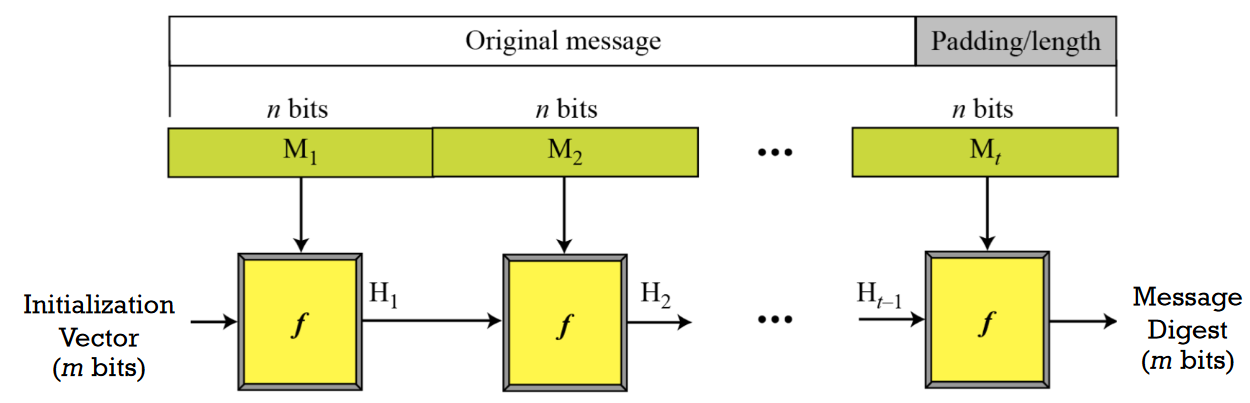
\includegraphics[width=0.7\linewidth]{Images/Chapter6/merkle}
	\caption{Hash function}
	\label{fig:merkle}
\end{figure}

Each stage of the Merkle structure takes two inputs: the $n$-bit block of the input message meant for that stage and the $m$-bit output of the previous stage. For the m-bit input, the first stage is supplied with a special $m$-bit pattern called the Initialization Vector ($IV$). The function $f$ that processes the two inputs, one $n$ bits long and the other m bits long, to produce an m bit output is usually called compression function. This is so since $n > m$, i.e. the output of the function $f$ is shorter than the length of the input message segment. The compression function $f$ may involve multiple rounds of processing of the two inputs to produce the output. The precise nature of $f$ depends on what hash algorithm is being implemented. The better $f$ is designed the better the hash function will be.

\section{The SHA family}

The last column refers to how many messages would have to be generated before two can be found with the same digest with a probability of 0.5 \ref{fig:sha}. As shown above, for a secure hash algorithm that has no security holes and that produces $n$-bit digests, one would need to come up with $2^{n/2}$ messages to discover a collision with a probability of $0.5$.
\begin{figure}
	\centering
	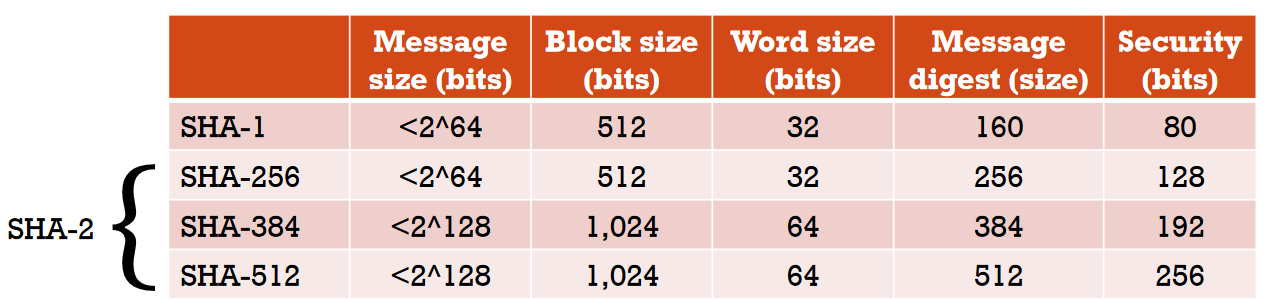
\includegraphics[width=0.7\linewidth]{Images/Chapter6/sha}
	\caption{SHA overview}
	\label{fig:sha}
\end{figure}

\subsection{SHA-1}
SHA-1 was cracked theoretically in the year 2005 by two different research groups, in 2017, SHA-1 was broken in practice \href{https://shattered.io}{shattered.io}.

\subsection{SHA-512}
SHA-512 has the following structure \ref{fig:merkle}.  It has 4 steps.

\subsubsection{SHA-512: Step 1}

This step consists in padding with length value. The goal is to make pad the message so that its length is an integral multiple of the block size = $512$ bits. Proviso: the last $128$ bits of the last block must contain a value that is the length of the message.
Even if the original message were by chance to be an exact multiple of $512$, one still needs to append another $512$-bit block at the end to make room for the $128$-bit message length integer. Leaving aside the trailing $128$ bit positions, the padding consists of a single $1$-bit followed by the required number of $0$-bits. 


\subsubsection{SHA-512: Step 2}

The goal is to initialize the hash buffer with IV. The hash buffer is represented by $8$ registers of $64$-bits that are labelled by a, b, c, d, e, f, g, h.

Generate the message schedule required for processing a 1024-bit block of the input message. The message schedule consists of 80 64-bit words: the first 16 of these words are obtained directly from the 1024-bit message block, the rest of the words are obtained by applying permutation and mixing operations to some of the previously generated words. 

\subsubsection{SHA-512: Step 3}

Apply round-based processing to each $1024$-bit input message block \ref{fig:sha-round2}.  There are $80$ rounds to be carried out for each message block. For round-based processing store the hash values calculated for the previous message block in temporary 64-bit variables a, b, c, d, e, f, g, h. In the $i$-th round, permute the values stored in these eight variables and, with two of the variables, mix in the message schedule words and a round constant. 
In the round-based processing of each input message block, the $i$-th round is fed the $64$-bit message schedule word $W_i$ and a special constant $K_i$. These constants are meant to be random bit patterns to break up any regularities in the message blocks. The round function consists of a sequence of transpositions and substitutions designed to diffuse to the maximum extent possible the content of the input message block \ref{fig:sha-round-function}.

\begin{figure}
	\centering
	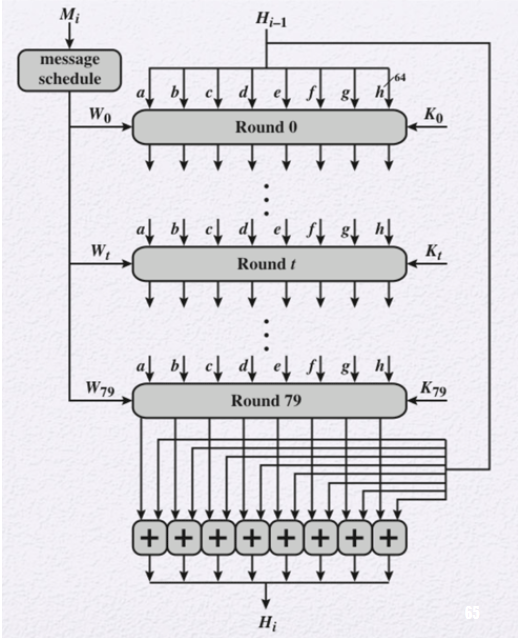
\includegraphics[width=0.7\linewidth]{Images/Chapter6/sha-round2}
	\caption{Function $f$}
	\label{fig:sha-round2}
\end{figure}

\subsubsection{SHA-512: Step 4}
After all the $t$ message blocks have been processed, the content of the hash buffer is the message digest.

\begin{figure}
	\centering
	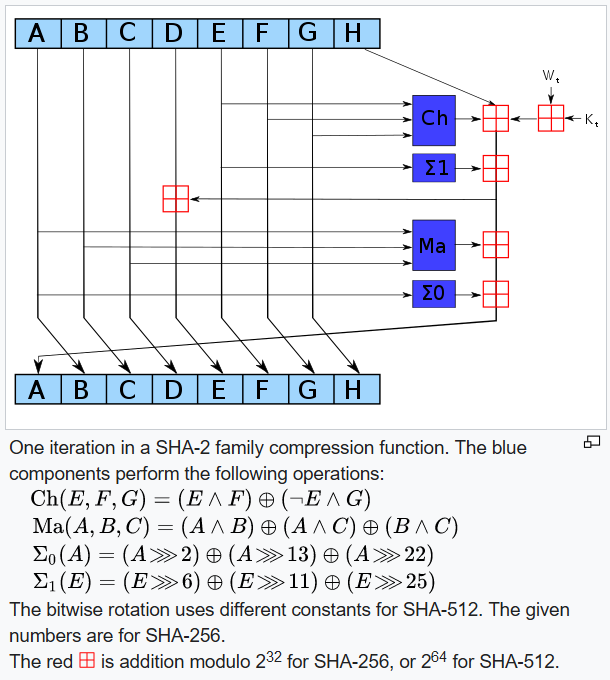
\includegraphics[width=0.7\linewidth]{Images/Chapter6/sha-round-function}
	\caption{SHA round function definition}
	\label{fig:sha-round-function}
\end{figure}


\section{Final remarks on hash functions}

Cryptographic hash functions should have three properties:
\begin{itemize}
	\item Pre-image resistance: given a digest $h(a)$ it is computationally infeasible to find $b$ such that $h(b) = h(a)$. Functions that lack this property are vulnerable to a pre-image attack
	\item Second pre-image resistance: given $a$ it is computationally infeasible to find $b$ such that $h(a) = h(b)$. Functions that lack this property are vulnerable to a second pre-image attack
	\item (Strong) Collision resistance: it is computationally infeasible to find a pair $(a,b)$ where $a \neq b$ such that $h(a) = h(b)$. For functions that lack this property a collision could be found via a birthday attack
\end{itemize}

In reality, hash functions are not close to one-way functions for which: it is easy to compute the digest, but it is computationally hard to compute a preimage.
There is no proof that one-way hash functions exist, or even concrete evidence that they can be constructed. Pragmatically, there are example hash functions (e.g., SHA-2 and SHA-3) that seem to be one-way hash functions that are easy to compute but we know of no easy way to find a preimage. 

Despite all these issues, for evaluating the theoretical security of hash functions, the random oracle model is used. A random Oracle is a function that gives fixed length output.  If it is the first time that it receives a particular input, it gives random output. If it already has received the input, it will repeat the corresponding output. This is the ideal strongly collision resistant function.  It can be used to prove security of encryption/signing under the assumption that the functions used behave like a random oracle. This is usually treated as strong evidence rather than a real proof. The evidence falls if weaknesses are found in the functions used.

\section{Application to cryptocurrencies}
Cryptocurrency is a digital currency in which encryption techniques are used to regulate the generation of units of currency and verify the transfer of funds, operating independently of a central bank \ref{fig:crypto}.

\begin{figure}
	\centering
	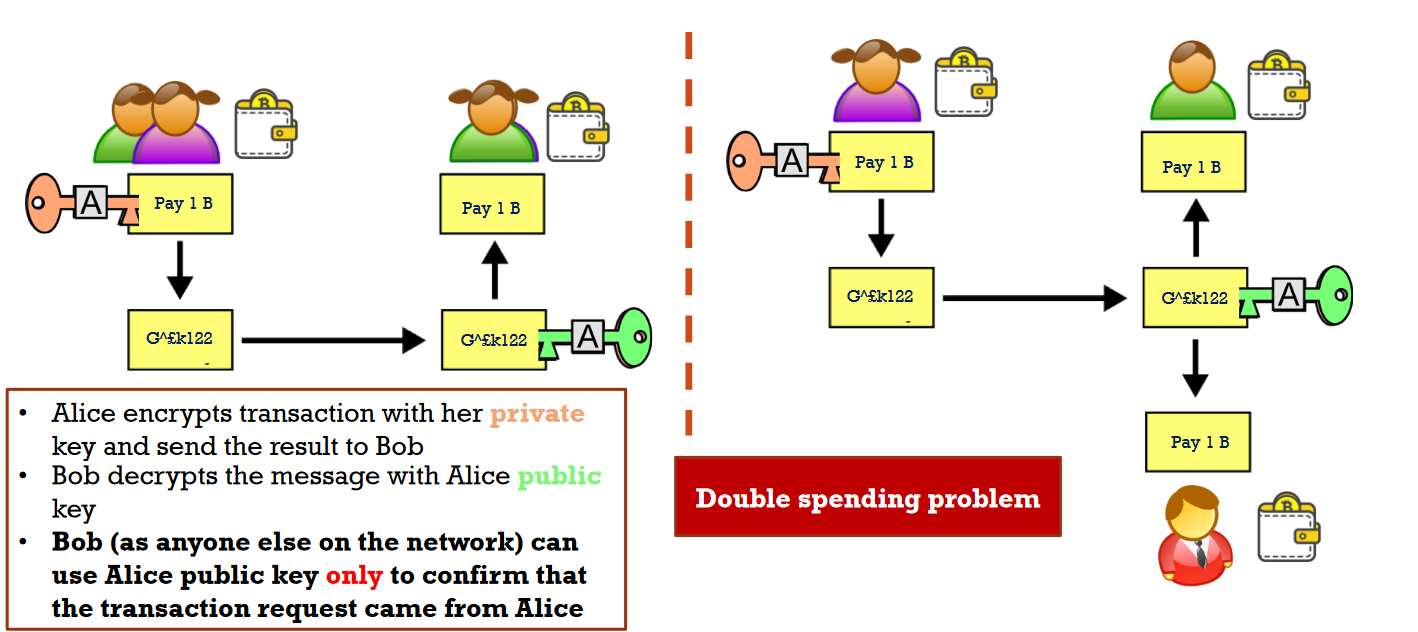
\includegraphics[width=0.7\linewidth]{Images/Chapter6/crypto}
	\caption{A transaction in the blockchain}
	\label{fig:crypto}
\end{figure}

The solution of the double spending problem is: mining. Mining is the process of issuing bitcoins. By proof of work we mean solving mathematical puzzles based on the notion of (cryptographic) hash function. Example find the number appended to "Hello, world!" that gives an hash that starts with 4 zeros (e.g. SHA256("Hello, world!4250") = 0000c3af42...). Since there is no way of predicting what the output will be, one has to guess. While it is hard to find a solution for the puzzle, it is easy to verify that the solution is correct. The mines that finds the correct solution gets rewarded bitcoins.

Hashing finds extensive use in crypto currency algorithms:
\begin{itemize}
	\item Used in the creation of bitcoin addresses to improve security and privacy.
	\item Proof-of-work calculations for mining a new coin
	\item Authenticate ownership of coins
	\item Establish a protocol for transferring the ownership from one node to another in a crypto currency network
	\item Create a protection against the double spending problem: no node should be able to sell the same coin to multiple other nodes in the network
\end{itemize}

Coins in cryptocurrencies are rare software object. The requirements are:
it must be extremely difficult to produce the object and it must be extremely easy to verify that it was extremely difficult to produce the object.

Bitcoin blockchain can be thought of as a decentralized database that is managed by distributed computers on a peer-to-peer network. Each peer maintains a copy of the ledger: updates and validations are reflected in all copies simultaneously.  A consensus algorithm is a process used to achieve agreement on a single data value among distributed processes or systems. Consensus algorithms are designed to achieve reliability in a network involving multiple unreliable nodes. Although any party can submit a chain of blocks to the ledger, the amount of computing resources required to fake consensus is too great to make it worthwhile to a dishonest party \ref{fig:blockchain}. 
The notion of a block as a set of transactions and, even more importantly, the notion a blockchain that is used to implicitly embed in each block a hash of all the previous transactions carried out so far. This provides security against the double spending problem and makes it possible to use crypto currencies in a manner similar to real currencies.  \footnote{TODO: Slide 90..111 10-HASH-2p.pdf}.

\begin{figure}
	\centering
	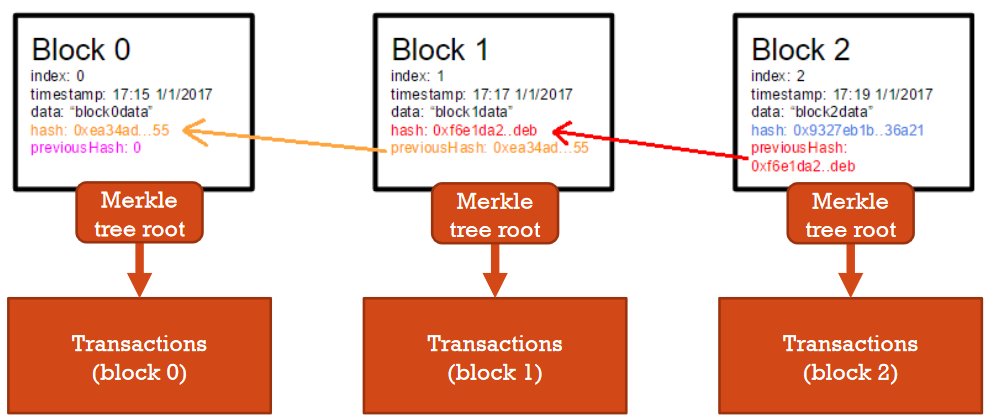
\includegraphics[width=0.7\linewidth]{Images/Chapter6/blockchain}
	\caption{Blockchain data structure}
	\label{fig:blockchain}
\end{figure}



\section{Fault tolerant consensus}


A group of generals must decide whether to attack or retreat. Some generals may prefer to attack, while others prefer to retreat. The important thing is that every general agrees on a common decision, for a half-hearted attack by a few generals would be much worse than either a coordinated attack or a coordinated retreat. The problem is complicated by the presence of treacherous generals who may not only cast a vote for a suboptimal strategy, they may do so selectively. Example: if 9 generals are voting, 4 of whom support attacking while 4 others are in favor of retreat, the 9th general may send a vote of retreat to those generals in favor of retreat, and a vote of attack to the rest... The problem is complicated further by the generals being physically separated and having to send their votes via messengers who may fail to deliver votes or may forge false votes.

In the simplified version of this problem two generals need to agree on the time to attack. General 1 has to send a messenger across the enemy's camp that will deliver the time of the attack to General 2. There is a possibility that the messenger will get captured by the enemies and thus the message will not be delivered resulting in General 1 attacking while General 2 not. Even if the first message goes through, General 2 has to acknowledge that he received the message, so he sends a messenger back, thus repeating the scenario where the messenger can get caught. This extends to infinite chains of acknowledgements with generals unable to reach agreement.

Byzantine Fault Tolerance is the characteristic which defines a system that tolerates the class of failures that belong to the Byzantine Generals Problem.
Bitcoin is Byzantine Fault Tolerant by solving the Byzantine Generals Problem by using the Proof-of-Work approach.